{\begin{a3pages}
% ---------------------------------------------------------------------------- %
\section{Sensorplatine}
\label{sec:hw:sensorplatine}
% ---------------------------------------------------------------------------- %
    \setlength{\parindentbak}{\parindent}

    \noindent\adjustbox{valign=t}{\begin{minipage}{135mm}
        Das  Sensorboard  besteht  aus  einer   CPU, welche  alle  Komponenten
        koordiniert, einem  Modulator und einem Demodulator  zur Kommunikation
        und  einem  Buck-Konverter,  der  die  Netzspannung  f\"ur  das  Board
        transformiert.

        \setlength{\parindent}{\parindentbak}
        Als   CPU  dient   ein  Atmel   SAM  D09   (Bereich  3   in  Abbildung
        \ref{fig:sensor:schema:highlights}). Dieser  wird  verwendet, weil  er
        der g\"unstigste Prozessor  in seiner Klasse ist  und alle notwendigen
        Funktionen  mitbringt. Der   Mikrochip  hat  einen  12   Bit-ADC,  ein
        CRC-Modul,  eine  32  Bit  ARM-Architektur und  braucht  extrem  wenig
        Leistung.

        Zum  Speisen  des  Boards  wird ein  LMR16006  von  Texas  Instruments
        verwendet (Bereich 1 in Abbildung \ref{fig:sensor:schema:highlights}).
        Dieser kann  die gesamte  Spanne der Modulspannung  von \SI{12}{\volt}
        bis \SI{60}{\volt}  ohne Probleme auf  \SI{3.3}{\volt} transformieren,
        welche das Board versorgt.

        Als Modulator  dient ein Voltage  Controlled Oscillator (VCO)  auf dem
        74HC4640-Chip von Texas Instruments (Bereich  2).  Dieser kann mit der
        richtigen Beschaltung  Frequenzen von  wenigen Kilohertz  bis mehreren
        Megahertz erzeugen.

        Zum Demodulieren wird ein einfaches Tiefpassfilter mit einer Diode und
        einem Verst\"arker benutzt (Bereich 6).

        Die  Messung der  Versorgungsspannung  ist  mit einem  Spannungsteiler
        implementiert,    zu   finden    in    Bereich    4   von    Abbildung
        \ref{fig:sensor:schema:highlights}.

        Bereich  5  enth\"alt   zwei  LEDs  und  einen   Schalter,  welche  zu
        Statusangaben und Debuggen am Sensor direkt verwendet werden k\"onnen.

        Im Folgenden werden die einzelnen Teilschaltungen dokumentiert und die
        Komponentenwahl begr\"undet.

        \adjustbox{valign=t}{\begin{minipage}{0.475\textwidth}
            \centering
            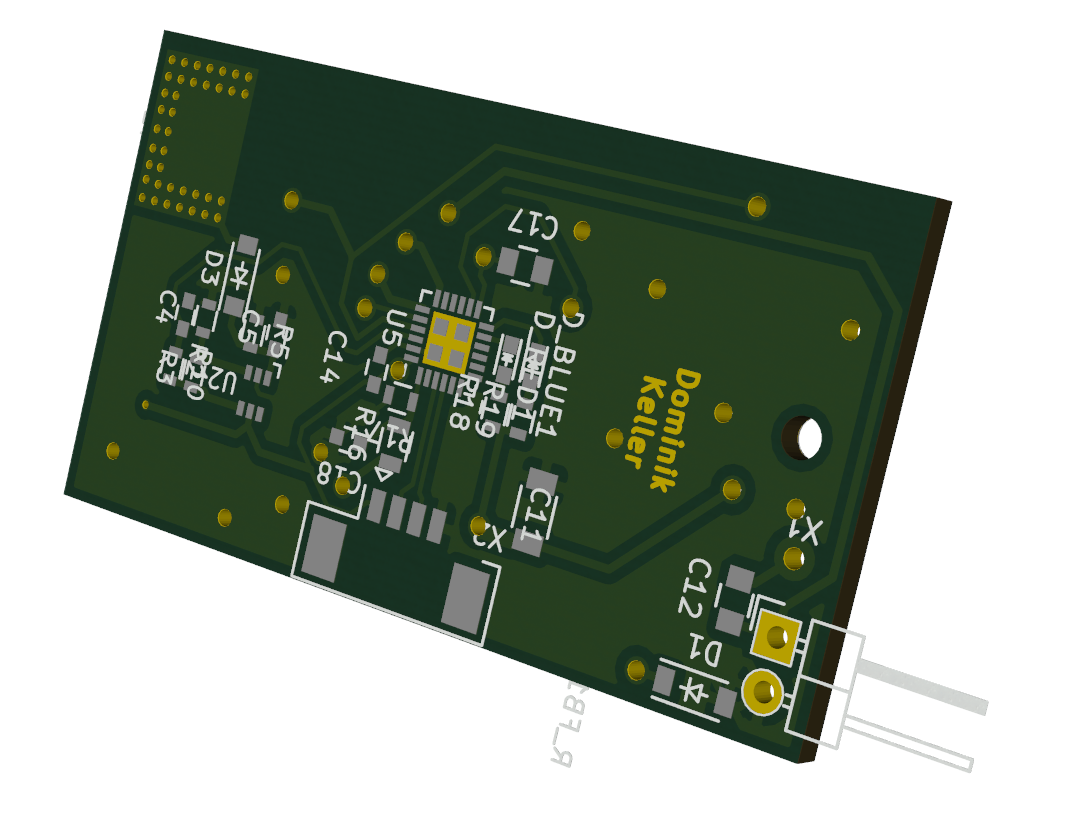
\includegraphics[width=0.9\textwidth]{images/sensor-pcb/sensor-3d-front.png}
            \figcaption[Sensor: Vorderseite PCB]{PCB, Vorderseite}
            \label{fig:sensor:pcb:front}
        \end{minipage}}
        \adjustbox{valign=t}{\begin{minipage}{0.475\textwidth}
            \centering
            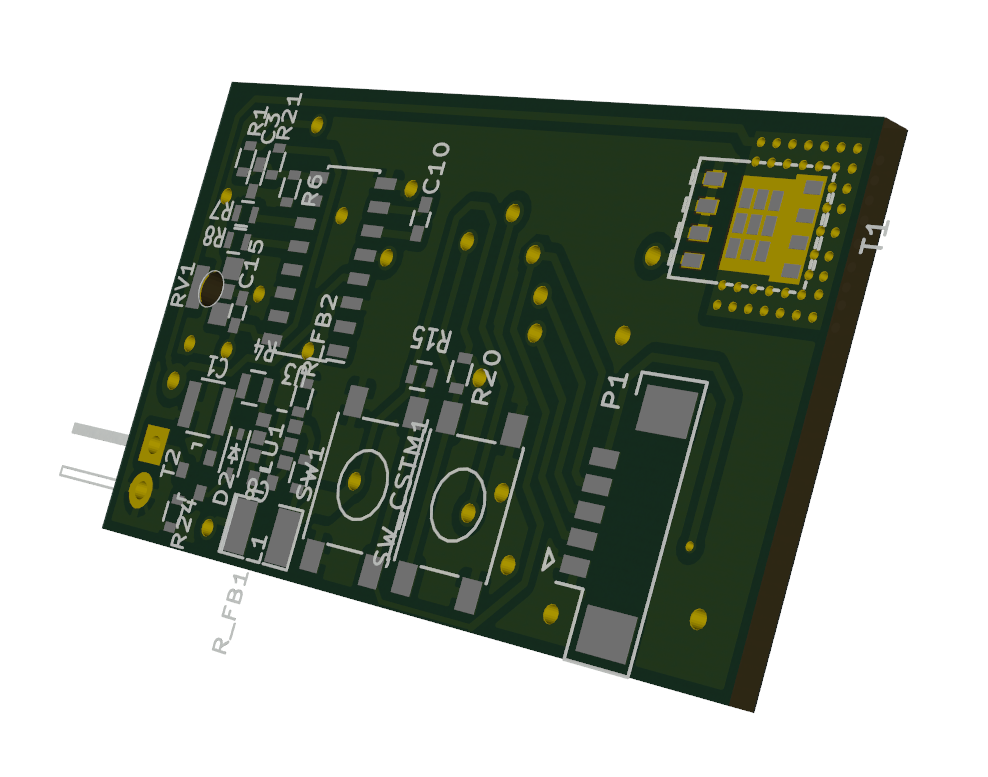
\includegraphics[width=0.9\textwidth]{images/sensor-pcb/sensor-3d-back.png}
            \figcaption[Sensor: R\"uckseite PCB]{PCB, R\"uckseite}
            \label{fig:sensor:pcb:back}
        \end{minipage}}
    \end{minipage}}
    \hspace*{15mm}
    \adjustbox{valign=t}{\begin{minipage}{195mm}
        \centering
        \includegraphics[width=\textwidth]{images/sensor-sch/sensor--sch--highlights.eps}%
        \figcaption[Schema Sensor, \"Ubersicht]{%
            Schema   des   \Sensor   s. Eine  Grossversion   ist   in   Anhang
            \label{app:chap:schemas}  zu  finden,   die  einzelnen  Baugruppen
            sind  in  den  folgenden  Abschnitten  beschrieben  und  gr\"osser
            abgebildet.%
        }
        \label{fig:sensor:schema:highlights}
    \end{minipage}}
\end{a3pages}}


% ---------------------------------------------------------------------------- %
\subsection{Speisung}
\label{subsec:hw:sensor:supply}
% ---------------------------------------------------------------------------- %

Die  Speisung  der  Schaltung   \"ubernimmt  ein  LMR16006. Er  verkraftet  am
Input   bis   \SI{63}{\volt}   und   sollte   so   die  an   handels\"ublichen
PV-Modulen    anliegenden   Spannungen    verkraften   (siehe    auch   Anhang
\ref{app:commercial:modules} auf  Seite \pageref{app:commercial:modules}).  Er
kommt auch  mit 4  Volt am  Eingang noch  klar. Da die  Versorgungsspannung im
Verlauf des  Tages zwischen \SI{12}{\volt} und  \SI{60}{\volt} schwanken kann,
ist der LMR16006 soweit bestens f\"ur unsere Schaltung geeignet.

Er  hat einen  sehr konstanten  Wirkungsgrad von  70 bis  80 Prozent,  je nach
Speisespannung.

Der  LMR16006 kann  maximal  \SI{600}{\milli\ampere}  liefern, was  ausreicht,
wenn  man   einen  genug  grossen  Pufferkondensator   f\"ur  Leistungsspitzen
einbaut   (\SI{10}{\micro\farad}  in   unserem  Fall,   rechts  in   Abbildung
\ref{fig:hw:sensor:speisung}).

Zudem  hat  dieser  Spannungsregler  einen  typischen  Quiescent  Current  von
nur  \SI{28}{\micro\ampere}. Damit  ist  er  auch  extrem  stromsparend.   Die
Beschaltung  wurde  nach   Empehlung  des  Datenblatts  \cite{ref:ti:lmr16006}
gew\"ahlt,  welche   garantiert,  dass  Powerspikes  gut   abgefangen  werden.
$R_{\mathrm{FB1}}$  und  $R_{\mathrm{FB2}}$  wurden  im  Verh\"altnis  $1:3.3$
gew\"ahlt, da \SI{3.3}{\volt} die Spannung ist, die wir am Ausgang anstreben.

Der Active  Low Shutdown Pin wird  dauernd auf High gezogen,  damit der Regler
immer an ist sobald am Eingang Spannung anliegt.

Damit die  Montage einfacher  ist, ist ein  Verpolungsschutz eingebaut. Dieser
besteht aus einem P-Fet, einer  Zenerdiode und einem Gate-Vorwiderstand (linke
Seite in Abbildung \ref{fig:hw:sensor:speisung}).

\vspace*{2em}

\begin{figure}[h!t]
    \centering
    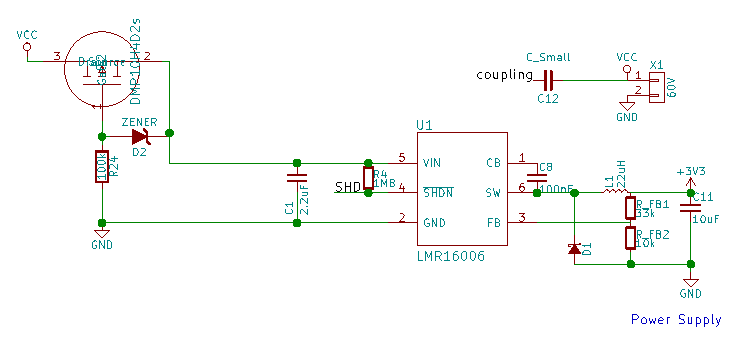
\includegraphics[width=1\textwidth]{images/sensor-sch/sensor--sch--supply.eps}
    \caption[Sensor: Schema Speisung]{Speisung Sensor}
    \label{fig:hw:sensor:speisung}
\end{figure}


% ---------------------------------------------------------------------------- %
\clearpage
\subsection{Transmitter}
\label{subsec:hw:sensor:transmitter}
% ---------------------------------------------------------------------------- %

Der  Transmitter  besteht  aus  einem   einfachen  VCO,  der  das  Signal  auf
die  Spannungsversorgung aufmoduliert.   Daf\"ur  wird am  $VCO_{\mathrm{in}}$
mithilfe eines Spannungsteilers eine fixe Spannung angelegt. Mit der korrekten
Wahl von \code{R7},  \code{R8} und \code{C10} kann  die Resonanzfrequenz f\"ur
die Leitung erreicht werden, mit der  dann moduliert wird. Diese Werte sind so
gew\"ahlt,  wie es  die  Graphen im  Datenblatt \cite{ref:ti:cd54}  zeigen. Es
wird  eine Frequenz  von  \SI{20}{\mega\hertz}  ausgew\"ahlt. Das Signal  wird
moduliert, indem der UART \code{TX} Pin  direkt am \code{INH} Pin den VCO ein-
und  ausschaltet  und  somit  ein  On-Off  Keying zustande  bringt. Hier  ist
wichtig, dass der Pin Active High ist.

\begin{figure}[h!t]
    \centering
    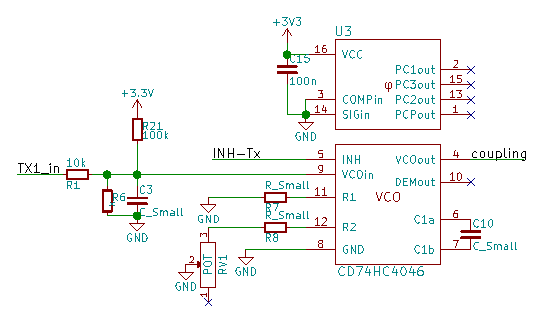
\includegraphics[width=0.70\textwidth]{images/sensor-sch/sensor--sch--transmitter.eps}
    \caption[Sensor: Schema Transmitter]{Transmitter Sensor}
\end{figure}


% ---------------------------------------------------------------------------- %
\subsection{Microcontroller}
\label{subsec:hw:sensor:mcu}
% ---------------------------------------------------------------------------- %

\begin{wrapfigure}{r}{0.6\textwidth}
    \centering
    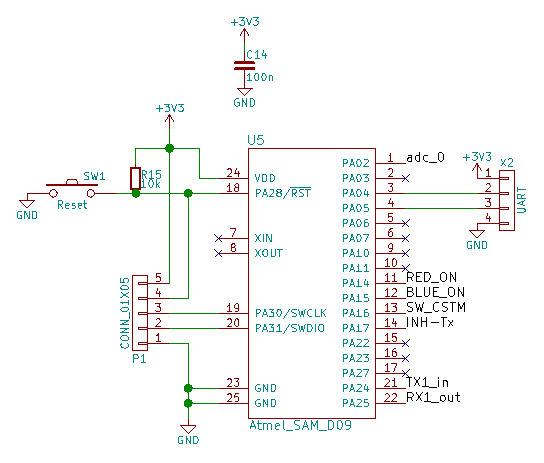
\includegraphics[width=0.60\textwidth]{images/sensor-sch/sensor--sch--mcu.eps}
    \caption[Sensor: Schema Microcontroller]{Microcontroller Sensor}
\end{wrapfigure}

Der  Mikrokontroller  braucht  bis  auf  einen  Pull-Up-Widerstand  am  Active
Low  Reset und  einem  Stabilisierungskondensator  an der  Spannungsversorgung
keine  spezielle  Beschaltung. Der  Mikrochip  ist  so  beschaltet,  dass  die
beiden  UART-Linien  verf\"ugbar sind;  eine  zum  Senden \"uber  die  Leitung
und  eine  zum   Debuggen. Ebenfalls  zu  einem  Stecker   verbunden  ist  die
Programmierschnittstelle (SWD). Das Datenblatt  ist unter \cite{ref:atmel:cpu}
verf\"ugbar.



% ---------------------------------------------------------------------------- %
\clearpage
\subsection{Spannungsmessung}
\label{subsec:hw:sensor:voltageSense}
% ---------------------------------------------------------------------------- %

Der  Spannungsteiler  ist  so  eingestellt, dass  am  ADC-Pin  \SI{3.3}{\volt}
anliegen,  wenn  bei  der Spannungsversorgung  \SI{60}{\volt}  anliegen.   Der
Kondensator \code{C18} dient der Gl\"attung des Signals.

\begin{figure}[h!t]
    \centering
    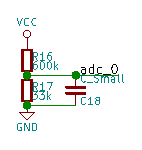
\includegraphics[width=0.25\textwidth]{images/sensor-sch/sensor--sch--sensor.eps}
    \caption[Sensor: Schema Spannungsmessung]{Spannungsmessung Sensor}
\end{figure}


% ---------------------------------------------------------------------------- %
\subsection{Interface}
\label{subsec:hw:sensor:interface}
% ---------------------------------------------------------------------------- %

\begin{figure}[h!t]
    \centering
    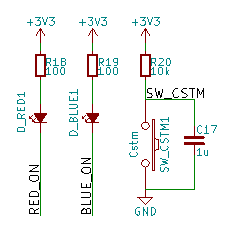
\includegraphics[angle=-90,width=0.4\textwidth]{images/sensor-sch/sensor--sch--interface.eps}
    \caption[Sensor: Schema Interface]{Interface Sensor}
\end{figure}

Am   Sensor  sind   zwei  LEDs   und  ein   Schalter  angebracht,   welche  zu
Statusanzeigen  und zum  Debuggen  benutzt werden  k\"onnen. In der  aktuellen
Firmware-Version  werden  die  LEDs   getoggled,  um  korrektes  Funktionieren
des  Sensors anzuzeigen  (siehe Abschnitt  \ref{subs:Statusanzeige} auf  Seite
\pageref{subs:Statusanzeige}).

% ---------------------------------------------------------------------------- %
\clearpage
\subsection{Empf\"anger}
\label{subsec:hw:sensor:receiver}
% ---------------------------------------------------------------------------- %

Der   Empf\"anger  ist   ein  einfaches   Tiefpassfilter.   Zuerst   wird  das
Eingangssignal,  welches  noch  moduliert   ist,  durch  die  Diode  \code{D3}
gleichgerichtet. Ein dahinter  geschalteter Tiefpass  sorgt daf\"ur,  dass das
Signal gegl\"attet wird. Da  dieses Signal durch Verluste auf  der Leitung und
\"uber der Diode eine viel zu kleine Amplitude hat, wird es zus\"atzlich durch
einen nicht invertierenden Opamp verst\"arkt.

\begin{figure}[h!t]
    \centering
    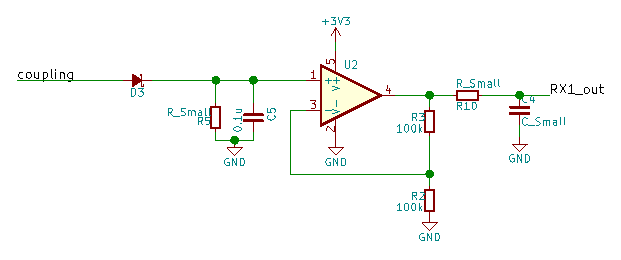
\includegraphics[width=0.9\textwidth]{images/sensor-sch/sensor--sch--receiver.eps}
    \caption[Sensor: Schema Empf\"anger]{Empf\"anger Sensor}
\end{figure}
